\documentclass{article}
\usepackage{graphicx}
\usepackage{pdflscape}
\usepackage{rotating}
\title{Core Circuit Model }
\author{Joshua Resnick}
\setlength\parindent{0pt}
\begin{document}
\maketitle


The model is built up in the following way. The core is modeled as 4 delay segments with the same characteristic impedance (1.55 ohms in this case) and 3 resistors. The three resistors represent the heated and unheated parts of the core - the middle resistor represents the part of the core heated by the cartridge heater. The output transmission line is just a delay with an impedance, and the termination resistor is just an ideal resistor. The respective delays of the core and output line can be measured from the respective waveform, so these are not really a degree of freedom. If RCore1 to RCore3 are all set to be equal (i.e. not modelling the variability in resistance across the core) then RCoreTotal collapses to a single degree of freedom. Likewise, we can set the impedance parameter for Core1, Core2, and Core3 to be equal. This gives us the following 4 degrees of freedom:
CoreZ, RCore, OutputLineZ, and RTerm.

RCore and RTerm dominate the amplitude components of the output, so they can be independently tuned by matching waveform amplitudes. So, I think we are primarily dealing with CoreZ and OutputLineZ as the tune-able variables. 


\begin{sidewaysfigure}
[h]
\begin{center}
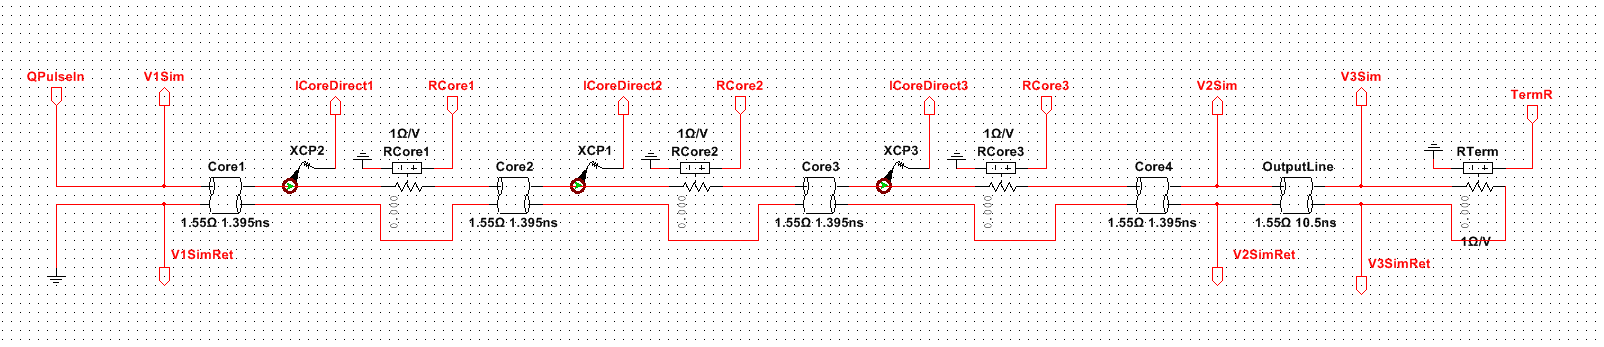
\includegraphics[scale=0.4]{image.png} 
\caption{Core Circuit Model}%
\end{center}
\end{sidewaysfigure}


\end{document}
